
\documentclass[11pt]{article}
\usepackage{listings}
\usepackage[utf8]{inputenc}
\usepackage{amsfonts,amsmath,amssymb}
\title{\textbf{How to CUSUM under normal distribution}}
\author{Pierre Ludmann}
\usepackage{graphicx}

\begin{document}

\maketitle

\section{The general formula in off-line view}

Set
\[L_k=\ln\left[\frac{\left(\sup_{\theta_0}\prod_{i=1}^{k-1}p_{\theta_0}(y_i)\right)\left(\sup_{\theta_1}\prod_{i=k}^Np_{\theta_1}(y_i)\right)}{\sup_{\tilde\theta}p_{\tilde\theta}(y_i)}\right]\]
where the $y_i$ are the $i$th observation of $N$.
And
\[L=\max_{1\le k\le N}L_k\]
If \[L\ge h\] with $h$ a certain threshold then there is a rupture in \[t_0=\arg\max_{1\le k\le N}L_k\]

A interpretation of this whole formula is quite simple : trying to get the best distribution assuming there is a change, if the maximal difference is significant the hypothesis test is passed at the time of maximum.

\section{Solve the sup}

To define a gaussian distribution, one just requires a mean $\mu$ and a standard-deviation $\sigma$. Then $\theta$ is one either or both.

Whatever the pick, one needs to get three sup : it represents a complex problem to compute. That's why we take advantage from the normal distribution.
Let divide a $L_k$, thanks to the fact that $\ln\sup f=\sup\ln f$, in
\[L_k=\frac{\sup_\theta F^k_0(\theta)\sup_\theta F^k_1(\theta)}{\sup_\theta\tilde F^k(\theta)}\]
Actually $F^k_0$, $F^k_1$ and $\tilde F^k$ are roughly the same and similar to
\[F(\theta)=\sum_{i=1}^n\ln p_\theta(y_i)=\sum_{i=1}^n\left[-\ln(\sigma\sqrt{2\pi})-\frac 12\left(\frac{y_i-\mu}\sigma\right)^2\right]\]
\[F(\theta)=-n\ln(\sigma\sqrt{2\pi})-\frac 12\sum_{i=1}^n\left(\frac{y_i-\mu}\sigma\right)^2\]
Notice $F$ is coercive whatever $\theta$ so a mere differential give the sup :
\\

If $\theta=\mu$ then $\hat\mu=\frac 1n\sum_{i=1}^ny_i$\\

If $\theta=\sigma$ then $\hat\sigma=\frac 1n\sum_{i=1}^n(y_i-\mu)^2$ ~~~~where $\mu$ is a set constant\\

If $\theta=(\mu,\sigma)$ then $\begin{cases}\hat\mu=\frac 1n\sum_{i=1}^ny_i\\
\hat\sigma=\frac 1n\left[\sum_{i=1}^ny_i^2-(\sum_{i=1}^ny_i)^2\right]\end{cases}$

\section{Simplify $L_k$ expression}

Be ready for stories without words \emph{i.e.} formula lines.

\subsection{Mean change}

\[L_k=
\sum_{i=1}^{k-1}\left[-\ln(\sigma\sqrt{2\pi})-\frac 12\left(\frac{y_i-\mu_0}{\sigma}\right)^2\right]
+\sum_{i=k}^N\left[-\ln(\sigma\sqrt{2\pi})-\frac 12\left(\frac{y_i-\mu_1}{\sigma}\right)^2\right]\]
\[~~~~~~~~~~~~~~~~~~~~~~~~-\sum_{i=1}^N\left[-\ln(\sigma\sqrt{2\pi})-\frac 12\left(\frac{y_i-\tilde\mu}{\sigma}\right)^2\right]\]

\[L_k=
-\frac 1{2\sigma^2}\left[\sum_{i=1}^{k-1}(y_i-\mu_0)^2
+\sum_{i=k}^N(y_i-\mu_1)^2
-\sum_{i=1}^N(y_i-\tilde\mu)^2\right]\]

\[L_k=\frac 1{2\sigma^2}\left[(k-1)\mu_0^2+(N-k+1)\mu_1^2-N\tilde\mu^2\right]\]

It is already well-simplified but the abstract factor $\sigma$ remains so we will compute him a value cause we need to take the hypothesis test.

\subsection{Standard-deviation change}

\[L_k=
\sum_{i=1}^{k-1}\left[-\ln(\sigma_0\sqrt{2\pi})-\frac 12\left(\frac{y_i-\mu}{\sigma_0}\right)^2\right]
+\sum_{i=k}^N\left[-\ln(\sigma_1\sqrt{2\pi})-\frac 12\left(\frac{y_i-\mu}{\sigma_1}\right)^2\right]\]
\[~~~~~~~~~~~~~~~~~~~~~~~~-\sum_{i=1}^N\left[-\ln(\tilde\sigma\sqrt{2\pi})-\frac 12\left(\frac{y_i-\mu}{\tilde\sigma}\right)^2\right]\]

\[L_k=
-\frac 12\left[\frac 1{\sigma_0^2}\sum_{i=1}^{k-1}(y_i-\mu)^2
+\frac 1{\sigma_1^2}\sum_{i=k}^N(y_i-\mu)^2
-\frac 1{\tilde\sigma^2}\sum_{i=1}^N(y_i-\mu)^2\right]\]
\[~~~~~~~~~~~~~~~~~~~~~~~~+N\ln(\tilde\sigma)-(k-1)\ln(\sigma_0)-(N-k+1)\ln(\sigma_1)\]

\[L_k=N\ln(\tilde\sigma)-(k-1)\ln(\sigma_0)-(N-k+1)\ln(\sigma_1)\]

\subsection{Both change}

\[L_k=
\sum_{i=1}^{k-1}\left[-\ln(\sigma_0\sqrt{2\pi})-\frac 12\left(\frac{y_i-\mu_0}{\sigma_0}\right)^2\right]
+\sum_{i=k}^N\left[-\ln(\sigma_1\sqrt{2\pi})-\frac 12\left(\frac{y_i-\mu_1}{\sigma_1}\right)^2\right]\]
\[~~~~~~~~~~~~~~~~~~~~~~~~-\sum_{i=1}^N\left[-\ln(\tilde\sigma\sqrt{2\pi})-\frac 12\left(\frac{y_i-\tilde\mu}{\tilde\sigma}\right)^2\right]\]

\[L_k=
-\frac 12\left[\frac 1{\sigma_0^2}\sum_{i=1}^{k-1}(y_i-\mu_0)^2
+\frac 1{\sigma_1^2}\sum_{i=k}^N(y_i-\mu_1)^2
-\frac 1{\tilde\sigma^2}\sum_{i=1}^N(y_i-\tilde\mu)^2\right]\]
\[~~~~~~~~~~~~~~~~~~~~~~~~+N\ln(\tilde\sigma)-(k-1)\ln(\sigma_0)-(N-k+1)\ln(\sigma_1)\]

\[L_k=N\ln(\tilde\sigma)-(k-1)\ln(\sigma_0)-(N-k+1)\ln(\sigma_1)\]

Amazingly, there is no such difference between expecting a change in variance or in variance and mean.

\section{When stop}

One could procede by recursive dichotomy. So the question is : should I stop when don't reach the threshold? That is to say :
\[\text{If }L_{t_0}< h\text{ then }\max_{1\le k\le t_0}L'_k< h\text{ and }\max_{t_0\le k\le N}L''_k< h\]
where $t_0=\arg\max_{1\le k\le N}L_k$, $L'_k$ and $L''_k$ is the log-likelihood ratio about each side of $t_0$.

It will be true for any threshold \underline{iff}
\[L_{t_0}\ge\max_k\left\{L'_k,L''_k\right\}\]
Unfortunately it is merely false according the following signals :

\subsection{Mean change}

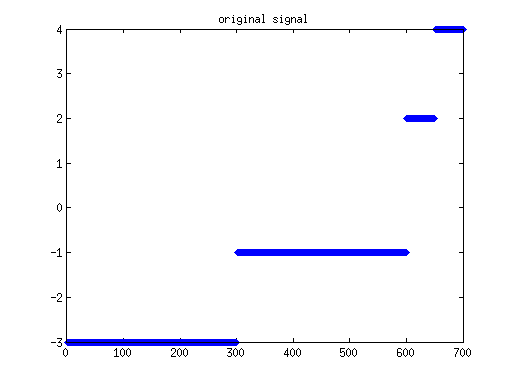
\includegraphics{stopmean0}
\hspace*{-5.3cm}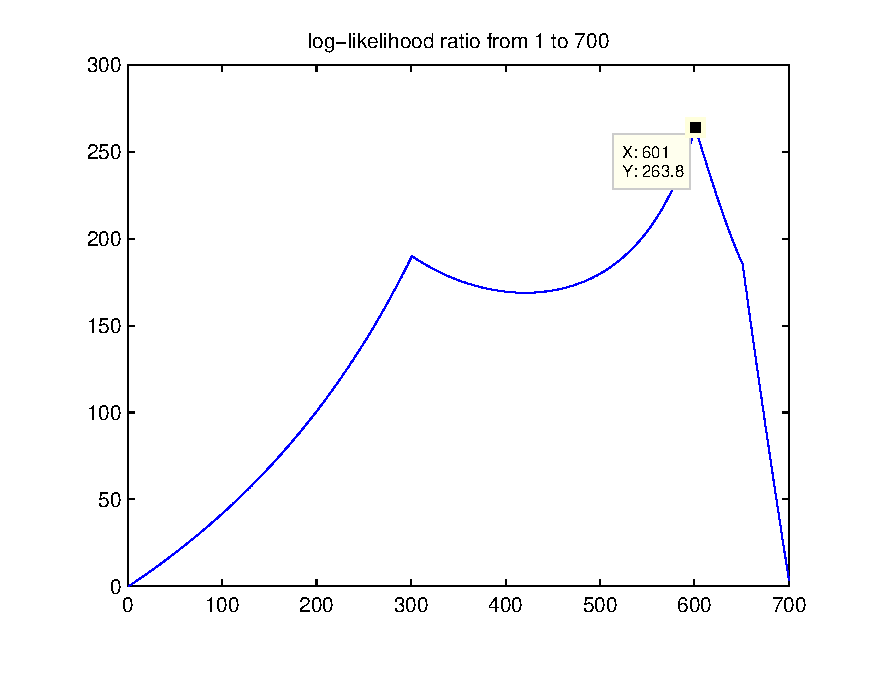
\includegraphics[width=0.89\linewidth]{stopmean1}
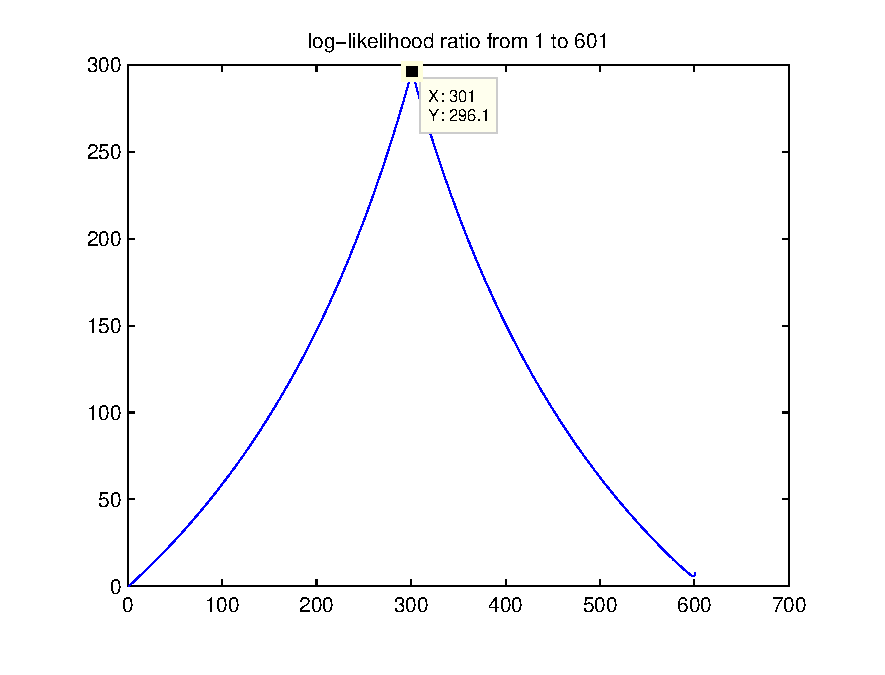
\includegraphics[width=0.89\linewidth]{stopmean2}

\subsection{Standard-deviation change}

  

\end{document}
